% !TEX program = lualatex
\documentclass[11pt]{article}

% -------- LuaLaTeX : polices et langue --------
\usepackage{fontspec}
\setmainfont{Latin Modern Roman}
\setsansfont{Tex Gyre Heros}
%\renewcommand{\familydefault}{\sfdefault} % force le sans serif par défaut
\usepackage{polyglossia}
\setdefaultlanguage{french}

% -------- Mise en page --------
\usepackage[a4paper,margin=1cm]{geometry}
\usepackage{multicol}
\usepackage{fancyhdr}
\pagestyle{empty}
\usepackage[most]{tcolorbox}

% -------- Mathématiques --------
\usepackage{amsmath,amssymb,mathtools}
% \usepackage{siunitx}
% \sisetup{locale=FR}

\usepackage{enumitem}
\setlist[itemize]{left=0pt}
\setlist[enumerate]{left=0pt, label=\textbf{\arabic*}.}

\usepackage{ProfCollege}
\usepackage{ProfMaquette}

%\usepackage{tabularray}
\usepackage{tabularx}

% -------- Divers --------
\newcommand{\ligne}{{\color{gray!60}\hrulefill}}

\setlength{\parindent}{0pt}

\begin{document}



\begin{Maquette}[DM]{
        Numero = 2, Code={}, Date = mardi 14 octobre 2025, Niveau = Troisième
    }


    \emph{Ce travail est à rédiger sur une feuille. L’exercice 3 n’est pas noté, il est à chercher et sera corrigé en classe. Le sujet n’est pas à rendre.}


    
    
    \begin{exercice}
        \brm{5}
        Le capitaine d’un navire possède un trésor constitué de 69 diamants, 1150 perles et 4140 pièces d’or.
        \begin{enumerate}
            \item Décomposer 69 puis 1150 et 4140 en produits de facteurs premiers.
            \item  Le capitaine partage équitablement le trésor entre les marins. Combien y-a-t-il de marins sachant que toutes les pièces, perles et diamants ont été distribués ?
            
        \end{enumerate}
    \end{exercice}
    
    \begin{exercice}
        \brm{5}
        Lucky Luke vient de tirer sur le chapeau d’Averell.\\
        On suppose que les deux cow-boys se tiennent perpendiculairement au sol.\\
        On sait que :
        \begin{itemize}
            \item Distance du sol au pistolet : PS = 1 m
            \item Distance parcourue par la balle : PC = 6,1 m
            \item Distance du pistolet à Averell : PA = 6 m
            \item Le triangle PAC est rectangle en A.
        \end{itemize}

        \begin{center}
            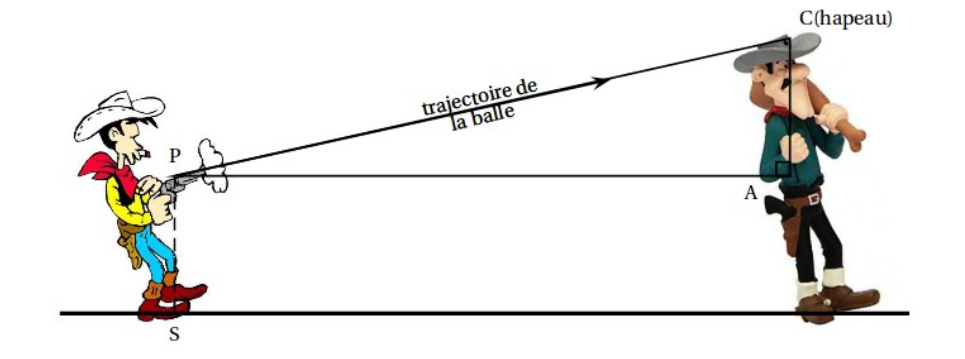
\includegraphics[width=.7\linewidth]{Images/DM2-LuckyLuke.png}
        \end{center}

        Calcule la taille d’Averell.
    \end{exercice}

    \newpage
    \begin{exercice}[BaremeTotal = false]
        Dans le repère ci-dessous, la largeur d’un carreau est de 10 pas.\\
        Au départ, le lutin se situe à l’\emph{origine} du repère et regarde \emph{vers la droite}.\\
        Trace ce que l’on obtient en lançant le programme suivant.

        \begin{center}
            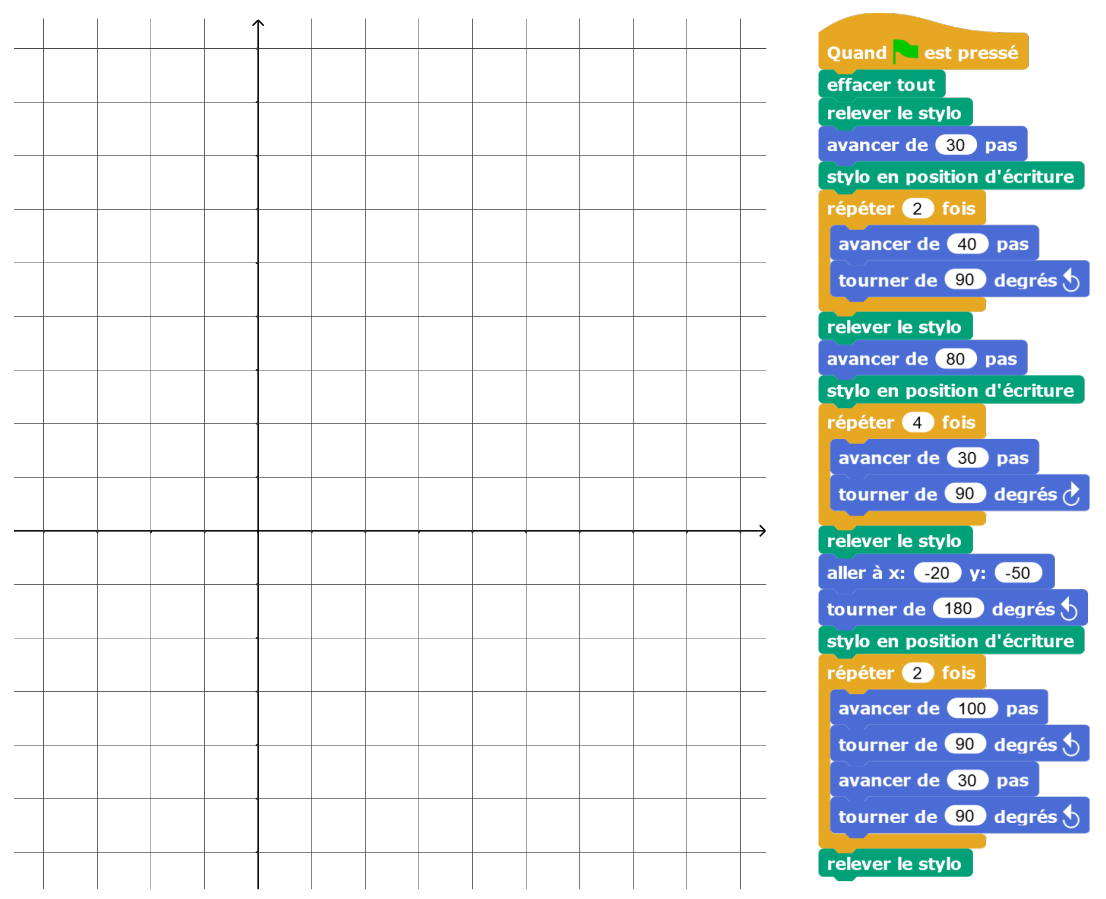
\includegraphics[width=\linewidth]{Images/DM2-scratch.png}
        \end{center}

        \textbf{aller à x: -20 et y: -50} signifie que le lutin se déplace au point de coordonnées (-20 ; -50).\\
        La direction dans laquelle il regarde ne change pas durant ce déplacement.
    \end{exercice}


\end{Maquette}


\end{document}